\chapter{The Bracket Polynomial}

Given two links or knots, one desires a way to tell if the two links are distinct. Since we can represent knots faithfully on a paper using knot diagrams, one can ask for a way to distinguish knots based on their diagrams. A \textit{link invariant} is a function of a link such that if the evaluation of the function on two links yields different outputs, then the links are distinct, i.e.\@ they are not ambient isotopic to each other. A link invariant is said to be \textit{complete} if it always gives different outputs for distinct links.

In this chapter, we shall a link invariant called the normalised bracket polynomial. It attaches each link a polynomial with coefficients from \(\Z[A, A^{-1}]\), where \(A\) and \(A^{-1}\) are some commuting variables. This invariant is not complete. It was discovered by Louis Kauffman in 1987~\cite{kauffmanstate1987, kauffmaninvariant}. The normalised version of this polynomial is equivalent to the Jones polynomial, which was discovered by Vaughn Jones in 1985 while working on the theory of operator algebras~\cite{jones}. The discovery of the Jones polynomial created a flurry of activity as relations between knot theory and mathematical physics were found. Several generalisations of the Jones/bracket polynomial were immediately found and some long standing problems in knot theory, such as the Tait conjectures were proved. The approaches of Jones and Kauffman are very different while defining their polynomials. While understanding the original route taken by Jones to define his polynomial requires the knowledge of the theory of von Neumann algebras, Kauffman takes an elementary, but powerful diagrammatic approach while defining his polynomial. In this chapter, we shall look at Kauffman's bracket polynomial using the so called \textit{state model}, as expounded in his book~\cite{kauffman}.

\section{State model}

Consider a crossing of an unoriented link as shown in \cref{fig:crossingresolution}. We designate local regions around a crossing a label \(A\) or \(B\) based on the following scheme. Walk along the underpass towards a crossing. The area on the left is assigned the label \(A\) and the area on the right the label \(B\). This assignment is unambiguous. We then `resolve' or `smoothen' or `split' the crossing in two ways, one way which connects the \(A\)-regions and another way which connects the \(B\)-regions. If we resolve a crossing such that \(A\)-regions are connected, then we attach the label \(A\) to the resolved diagram. The same holds for \(B\)-regions. Note that the resolution of the crossing happens only locally, i.e.\@ in an open ball around the crossing which does not intersect other crossings. Such an open ball exists due to the Hausdorff property of the plane.

\begin{figure}
	\centering
	\begin{tikzcd}
		{}& \KPAB \arrow[thick, dl]\arrow[thick, dr]& \\
		\KPAD   &  &  \KPAE
	\end{tikzcd}
	\caption{Resolution of a crossing with labels}\label{fig:crossingresolution}
\end{figure}

% \begin{figure}
%     \centering
% 	\includesvg{crossingresolution.svg}
% 	\caption{Resolution of a crossing.}
% 	\label{fig:crossingresolution}
% \end{figure}

We shall do this process recursively for all crossings to get a sets of Jordan curves in a plane with labels attached to them. Refer to \cref{fig:trefoilres} where we have carried this process for a trefoil.

\begin{figure}
    \centering
	\includesvg[width=\textwidth]{trefoilres.svg}
	\caption{Resolution of all crossings for a trefoil.}
	\label{fig:trefoilres}
\end{figure}

Each of the individual diagrams shown in curly brackets in \cref{fig:trefoilres} is referred to as a state. To each state are the labels \(A\) and \(B\) attached to it. We can construct the original link unambiguously using the states (and labels attached to them). We shall construct invariants of links by `averaging' over these states.

By averaging, we mean the following. Let \(L\) be a link and \(\sigma\) denote a particular state obtained after resolving all the crossings recursively. We denote the commutative product of the labels associated to that state by \(\braket<K|\sigma>\). For example, let \(K\) denote a right-handed trefoil, as shown in \cref{fig:trefoilres} and \(\sigma\) denote the following state.
\begin{figure}[H]
    \centering
	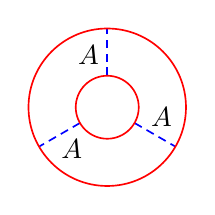
\begin{tikzpicture}
		\draw[line width=0.6pt, densely dashed, blue] (-30:0.4) -- (-30:1);
		\draw[line width=0.6pt, densely dashed, blue] (-150:0.4) -- (-150:1);
		\draw[line width=0.6pt, densely dashed, blue] (90:0.4) -- (90:1);
		\draw[line width=0.6pt, red] (0,0) circle [radius=1];
		\draw[line width=0.6pt, red] (0,0) circle [radius=0.4];
		\node (a) at (-10:0.7) {\(A\)};
		\node (a) at (-130:0.7) {\(A\)};
		\node (b) at (110:0.7) {\(A\)};
% 		\node (d) at (-1.5,0) {\(\sigma = \)};
	\end{tikzpicture}
\end{figure} We then have \[\left\langle\TREFOIL \Bigg\vert\hspace{2pt}\AAA\right\rangle = A^3.\] Let \(\norm{\sigma}\) denote one less than the number of loops in \(\sigma\). Thus, for the above state, we have \(\norm{\sigma} = 1-1=0\).

We define the bracket polynomial \(\langle L\rangle\) of a link \(L\) as follows. \[\langle L \rangle = \sum_\sigma\braket<L|\sigma> d^{\norm{\sigma}},\] where \(A\), \(B\) and \(d\) are commuting variables. The bracket polynomial is thus a function of \(A\), \(B\) and \(d\). \(\sigma\) runs over all the states of \(K\).

Thus, we calculate \(\braket<L|s>\) for each state for the trefoil to get
\begin{align*}
    \langle L\rangle &= A^3d^{2-1} + A^2Bd^{1-1} + A^2Bd^{2-1} + A^2Bd^{1-1}\\
					 &\phantom{=\,} + AB^2d^{2-1} + AB^2d^{2-1} + B^3d^{3-1}\\
	\langle L\rangle &= A^3d + 3A^2Bd^0 + 3AB^2d^1 + B^3d^2.
\end{align*}

\begin{thm}[Skein relation]
    \[\BB = A\BD + A^{-1}\BE.\]
\end{thm}

The diagrams in the above theorem should be regarded as local diagrams. We make changes to a diagram locally near the crossing. There exists an open topological ball around each crossing such that the ball does not intersect any other crossing and the diagram remains identical outside this ball.

The proof of the above theorem follows from the definition of \(\braket<L>\) and realizing that the states of a diagram are in one-to-one correspondence with the union of the diagrams with resolved crossings. The above identity is very important and we shall use it very often. For an example of a calculation of the bracket polynomial of a link, please refer to \cref{fig:hopflinkbracket}.

\begin{figure}
    \centering
	\includegraphics[width=\textwidth]{hopflinkbracket.png}
	\caption{Bracket polynomial calculation for the Hopf link}
	\label{fig:hopflinkbracket}
\end{figure}

\begin{thm}
	\[\Bintersection = AB \BE + AB\Bthirty + (A^2 + B^2)\BD.\]
\end{thm}
\begin{proof}
	\[\Bintersection = A\Bigl\langle\hspace{-3pt}\KPthirtyoneone\hspace{-3pt}\Bigr\rangle + B\Bigl\langle\hspace{-3pt}\KPthirtyonetwo\hspace{-3pt}\Bigr\rangle.\] This splits into \[\Bintersection = A\left[A\Bigl\langle\hspace{-2.5pt}\vcenter{\hbox{\KPthirtyonethree}}\hspace{-2.5pt}\Bigr\rangle + B\Bthirty\right] + B\left[A\Bigl\langle\hspace{-2.5pt}\vcenter{\hbox{\KPthirtyonefour}}\hspace{-2.5pt}\Bigr\rangle + B\Bigl\langle\hspace{-2.5pt}\vcenter{\hbox{\KPthirtyonefive}}\hspace{-2.5pt}\Bigr\rangle\right].\] Finally we have \[\Bintersection = AB \BE + AB\Bthirty + (A^2 + B^2)\BD.\]
\end{proof}
It is also clear that \[\Bigl\langle\hspace{-2pt}\plusoneu\Bigr\rangle = (Ad + B)\langle\lineone\rangle\] and \[\Bigl\langle\hspace{-2pt}\minusoneu\Bigr\rangle = (A + Bd)\langle\lineone\rangle.\] We also see that \[\left\langle\KPthirtyonesix\right\rangle = d\langle\lineone\rangle.\]

Let \(B = A^{-1}\) and \(d = -A^2 - A^{-2}\). We shall always use these substitutions from now on.

We see that \[\Bintersection = \BE.\] This illustrates the invariance under a type II move. But note that \[\Bigl\langle\hspace{-2pt}\plusoneu\Bigr\rangle = (-A^{-3})\langle\lineone\rangle\] and \[\Bigl\langle\hspace{-2pt}\minusoneu\Bigr\rangle = (-A^{3})\langle\lineone\rangle.\] This follows from substituting \(B = A^{-1}\) and \(d = -A^2 - A^{-2}\) in \(Ad + B\) to get \(-A^3\). This illustrates that the bracket polynomial is \textit{not} invariant under a type I move. Adding a twist multiplies the bracket by a factor of \(-A^3\) or \(-A^{-3}\), depending upon the type of the twist. This suggests that if we multiply by a compensatory factor, then we can possibly make it invariant under a type I move as well. We shall do this later using a normalisation factor.

Type II invariance of the bracket and the substitutions ensure that the bracket polynomial is invariant under a type III move as well.

\begin{thm}
	\[\Bigl\langle\hspace{-6.5pt}\KPthirtytwoone\hspace{-6.5pt}\Bigr\rangle = \Bigl\langle\hspace{-6.5pt}\KPthirtytwotwo\hspace{-6.5pt}\Bigr\rangle.\]
\end{thm}
\begin{proof}
	We have \[\Bigl\langle\hspace{-6.5pt}\KPthirtytwoone\hspace{-6.5pt}\Bigr\rangle = A\Bigl\langle\hspace{-6.5pt}\KPthirtytwofour\hspace{-6.5pt}\Bigr\rangle + B\Bigl\langle\hspace{-6.5pt}\KPthirtytwofive\hspace{-6.5pt}\Bigr\rangle.\] Using the type II moves, we have \[A\Bigl\langle\hspace{-6.5pt}\KPthirtytwothree\hspace{-6.5pt}\Bigr\rangle + B\Bigl\langle\hspace{-6.5pt}\KPthirtytwosix\hspace{-6.5pt}\Bigr\rangle = \Bigl\langle\hspace{-6.5pt}\KPthirtytwotwo\hspace{-6.5pt}\Bigr\rangle.\]
\end{proof}

We have thus found a regular isotopy invariant. A general principle is that once we have a regular isotopy invariant, we can suitably normalise it to make it ambient isotopy invariant. We know that writhe is an invariant of regular isotopy. Adding a positive twist increases the writhe by unit value and adding a negative twist decreases the writhe by unit value. As remarked earlier, we multiply the bracket by compensatory factor \(-A^3)^{-\w(K)}\) to define the normalised bracket polynomial. \[\kau(A, K) \coloneq (-A^3)^{-\w(K)} \langle K\rangle.\]

\begin{thm}
    The normalised bracket polynomial is an invariant of ambient isotopy.
\end{thm}
\begin{proof}
    Since both the writhe and the bracket are regular isotopy invariant, it follows at once that the normalised bracket is regular isotopy invariant as well. We need to check type I move invariance. Recall that \[\Bigl\langle\hspace{-2pt}\plusoneu\Bigr\rangle = (-A^{-3})\langle\lineone\rangle\] and \[\Bigl\langle\hspace{-2pt}\minusoneu\Bigr\rangle = (-A^{3})\langle\lineone\rangle.\] These identities combined with the behaviour of writhe under adding twists ensures type I invariance.
\end{proof}

\begin{thm}
	Let \(K^*\) denote the mirror image of the oriented link \(K\). Then we have that \(\langle K^*\rangle (A) = \langle K\rangle(A^{-1})\) and \(\kau(A, K^*) = \kau(A^{-1}, K)\).
\end{thm}
\begin{proof}
	Note that the link diagram of the mirror image of a link is obtained by switching all the crossings. This means that all the \(A\)'s and the \(A^{-1}\)'s get exchanged as well.
\end{proof}

We calculate the bracket polynomial for various knots and links in the appendix. In particular, we calculate the normalised bracket polynomial for a trefoil and and its mirror image. For the trefoil shown in \cref{fig:variousknots}, which is the left-handed trefoil knot, the normalised bracket polynomial turns out to be \(A^4 + A^{12} - A^{16}\) and the normalised bracket polynomial for its mirror image turns out to be \(A^{-4} + A^{-12} - A^{-16}\), as expected. But since the polynomials are different, we can conclude that a trefoil is \textit{not} ambient isotopic to its mirror image. The normalised bracket polynomial for the Whitehead figure eight knot turns out to be \(A^8 - A^4 + 1 - A^{-4} + A^{-6}\), which is symmetric in the powers of \(A\), indicating that the mirror image of the figure eight knot is identical to the original one. While this proof of the chirality of trefoil is elementary, this fact was originally proved by Max Dehn in 1914 using the newly discovered fundamental group~\cite[p.~200]{dehn}.



